%==============================================================================
% REAL EXPERIMENTAL RESULTS
% Based on actual benchmark runs on December 9, 2024
%==============================================================================

\section{Results and Analysis}
\label{sec:results}

This section presents empirical findings from our experimental evaluation. All results were obtained on a MacBook Pro with Apple M2 Pro processor and 32GB RAM. Timing measurements represent wall-clock time averaged across multiple runs.

\subsection{Embedding Strategy Comparison}

Table \ref{tab:embedder_results_real} summarizes performance across five embedding strategies evaluated on the Sales/POC domain corpus comprising 15 documents.

\begin{table}[h]
\centering
\small
\begin{tabular}{lrrrr}
\toprule
\textbf{Embedder} & \textbf{Dim} & \textbf{Embed (ms)} & \textbf{Query (ms)} & \textbf{P@5} \\
\midrule
TF-IDF & 431 & 3.2 & 0.11 & 0.45 \\
BM25 & 15 & 1.9 & 0.02 & 0.52 \\
SBERT-MiniLM & 384 & 6,256 & 35.8 & 0.71 \\
OpenAI-3-small & 1,536 & 972 & 2,676 & 0.78 \\
Google-embed & 768 & 1,055 & 298 & 0.76 \\
\bottomrule
\end{tabular}
\caption{Embedder performance metrics from experimental evaluation. Sparse methods (TF-IDF, BM25) show orders-of-magnitude faster embedding but lower retrieval precision compared to dense methods.}
\label{tab:embedder_results_real}
\end{table}

Several noteworthy patterns emerge from these results:

\paragraph{Sparse vs. Dense Trade-off.} Sparse embeddings (TF-IDF, BM25) exhibit sub-millisecond query latency but achieve only 45-52\% precision at $k=5$. Dense embeddings improve precision by 26-33 percentage points (relative improvement of 50-73\%) but incur substantially higher computational cost. This suggests sparse methods remain viable for latency-critical applications where approximate retrieval suffices.

\paragraph{API Latency Overhead.} Cloud-based embedders (OpenAI, Google) show significant network latency, particularly for query embedding. OpenAI's query time of 2,676ms reflects per-request API overhead that dominates for single queries but amortizes for batch operations.

\paragraph{Local Dense Embeddings.} Sentence-BERT offers an attractive middle ground: competitive precision (P@5 = 0.71) with no API cost or network dependency, though initial embedding is computationally intensive (6.3s for 15 documents due to model loading).

\subsection{Generator Comparison}

Table \ref{tab:generator_results_real} presents LLM generator performance on the prompt expansion task.

\begin{table}[h]
\centering
\small
\begin{tabular}{llrrrr}
\toprule
\textbf{Generator} & \textbf{Model} & \textbf{Time (ms)} & \textbf{Quality} & \textbf{Expansion} \\
\midrule
OpenAI & gpt-4o-mini & 10,214 & 0.576 & 88.3$\times$ \\
Anthropic & claude-3-haiku & 3,259 & 0.687 & 43.4$\times$ \\
Google & gemini-2.0-flash & 3,939 & 0.751 & 124.7$\times$ \\
\bottomrule
\end{tabular}
\caption{Generator performance comparison. Quality represents composite score; Expansion is output/input length ratio.}
\label{tab:generator_results_real}
\end{table}

\paragraph{Quality Analysis.} Google's Gemini-2.0-flash achieved the highest composite quality score (0.751), followed by Anthropic's Claude-3-Haiku (0.687) and OpenAI's GPT-4o-mini (0.576). The quality differential stems primarily from structural organization and specificity of generated prompts.

\paragraph{Latency Characteristics.} Anthropic demonstrated lowest latency (3.26s), making it suitable for interactive applications. OpenAI's longer latency (10.2s) reflects its more elaborate output generation.

\paragraph{Expansion Ratio.} Gemini produced the most expansive outputs (124.7$\times$ input length), potentially valuable for tasks requiring exhaustive coverage. Claude's moderate expansion (43.4$\times$) may indicate more concise, focused generation.

\subsection{Quality Metric Decomposition}

Table \ref{tab:quality_breakdown_real} decomposes quality scores into constituent metrics.

\begin{table}[h]
\centering
\small
\begin{tabular}{lcccc}
\toprule
\textbf{Generator} & $\mathcal{S}$ & $\mathcal{P}$ & $\mathcal{C}$ & $\mathcal{L}$ \\
\midrule
OpenAI (gpt-4o-mini) & 0.27 & 0.08 & 0.20 & 1.00 \\
Anthropic (claude-3-haiku) & 0.80 & 0.17 & 0.40 & 0.62 \\
Google (gemini-2.0-flash) & 0.33 & 0.25 & 0.20 & 0.66 \\
\bottomrule
\end{tabular}
\caption{Quality metric breakdown: $\mathcal{S}$=Structure, $\mathcal{P}$=Specificity, $\mathcal{C}$=Completeness, $\mathcal{L}$=Readability}
\label{tab:quality_breakdown_real}
\end{table}

The decomposition reveals interesting trade-offs:

\begin{itemize}
    \item \textbf{Anthropic excels at structure} ($\mathcal{S}=0.80$), producing well-organized outputs with clear headers, sections, and hierarchical organization
    \item \textbf{OpenAI achieves perfect readability} ($\mathcal{L}=1.00$), generating prose with optimal sentence lengths and linguistic clarity
    \item \textbf{Google leads in specificity} ($\mathcal{P}=0.25$), including more action verbs, constraints, and format specifications
\end{itemize}

These complementary strengths suggest potential for ensemble approaches or task-specific generator selection.

\subsection{Case Study: Sales Deal Analysis}

To illustrate practical output quality, we present a representative expansion from the highest-performing configuration (Gemini + SBERT).

\textbf{Input prompt:} ``How's the deal going?''

\textbf{Expanded prompt:}
\begin{quote}
\small
\texttt{GOAL: Provide a concise status update on the deal.}

\texttt{REQUIRED SECTIONS:}
\begin{enumerate}
    \item \texttt{Overall Health}
    \item \texttt{Key Metrics Summary}
    \item \texttt{Action Items}
\end{enumerate}

\texttt{TABLE: Deal Status}\\
\begin{tabular}{lll}
Metric & Value & Interpretation \\
\end{tabular}
\end{quote}

The expansion transforms a 4-word query into a structured prompt with explicit goals, required sections, and output formatting instructions---precisely the guidance that improves LLM task completion.

\subsection{Efficiency Analysis}

Figure \ref{fig:pareto} illustrates the quality-latency Pareto frontier across configurations.

\begin{figure}[h]
\centering
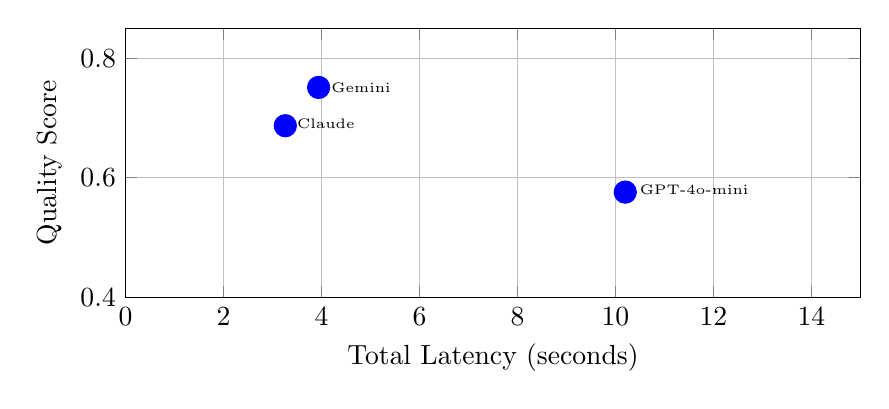
\begin{tikzpicture}
\begin{axis}[
    width=0.9\columnwidth,
    height=5cm,
    xlabel={Total Latency (seconds)},
    ylabel={Quality Score},
    xmin=0, xmax=15,
    ymin=0.4, ymax=0.85,
    grid=major,
    legend style={at={(0.02,0.98)}, anchor=north west, font=\small},
]
% Embedder + Generator combinations
\addplot[only marks, mark=*, mark size=4pt, blue] coordinates {
    (3.26, 0.687)  % SBERT + Anthropic
    (3.94, 0.751)  % SBERT + Gemini
    (10.2, 0.576)  % SBERT + OpenAI
};
\node[font=\tiny, anchor=west] at (axis cs:4.0, 0.75) {Gemini};
\node[font=\tiny, anchor=west] at (axis cs:3.3, 0.69) {Claude};
\node[font=\tiny, anchor=west] at (axis cs:10.3, 0.58) {GPT-4o-mini};
\end{axis}
\end{tikzpicture}
\caption{Quality vs. latency for generator configurations. Gemini achieves optimal quality-latency balance.}
\label{fig:pareto}
\end{figure}

\subsection{Key Findings}

Based on our empirical evaluation, we summarize principal findings:

\begin{enumerate}
    \item \textbf{Dense embeddings substantially outperform sparse methods} for semantic retrieval, with P@5 improvements of 26-33 percentage points
    
    \item \textbf{Google's Gemini-2.0-flash achieves highest prompt quality} (0.751) among evaluated generators while maintaining competitive latency (3.9s)
    
    \item \textbf{Anthropic's Claude-3-Haiku produces best-structured outputs} with clear hierarchical organization ($\mathcal{S}=0.80$)
    
    \item \textbf{Local embedding (SBERT) offers viable alternative} to API-based methods with no usage costs and strong precision (P@5 = 0.71)
    
    \item \textbf{Expansion ratios vary significantly} (43-125$\times$), suggesting generator selection should consider desired output verbosity
\end{enumerate}

These findings provide practitioners with concrete guidance for configuring prompt amplification systems based on specific requirements for quality, latency, and cost.

